\documentclass{./cls/hw}
\usepackage{graphicx,mathtools,inputenc,xspace, bm, amssymb,circuitikz}

\title{On-Site Homework 10}
\course{ECEN 2420}
\author{$\boxed{\text{Patrick Harrington}}$}

\begin{document}
\maketitle
\section*{Introduction}
The power amplifier and transmit mixer were constructed and analyzed. The
power amplifier is the final amplification stage prior to the Harmonic
filter, with an output designed to be around 2 Watts. The Transmit mixer is
designed to combine the signal from the VFO and the Transmit oscillator.

%\begin{figure}[h!]\label{Norcal40A}
\centering
  \begin{circuitikz}[american voltages] \draw
%  (0,0) node[anchor=east] {}
%  to[ sV ] (2,0)
  ;\end{circiuitikz}
\end{figure}

\begin{figure}[h!]\label{Norcal40A}
  \centering
  \begin{circuitikz}[american voltages] \draw
  (0,0) node[anchor=east] {Key}
    to[ sV=Tx Osc., o- ] (2,0)
    (3,0) node[mixer] (txmix) {}
      (txmix.in 1) node[left] {}
      (txmix.in 2) node[below] {}
      (txmix.out)  node[right] {}

    (6,0) node[buffer] (buf) {}
    (8,0) node[buffer] (drv) {}
    (10,0) node[buffer] (pow) {}
    (13,-0.25) node[european and port] (harmfilt) {h}
    (13,-0.25) node[antenna] (ant) {}
   
    (3,-2) node[] (VFO1) {}
    (7,-2) node[] (VFO2) {}
    (VFO1) to[short ,i=2.1] (txmix.in 2) 
    (VFO1) to[sV=VFO] (VFO2)


      %Connections
     (2,0) to[short, i=4.92] (txmix.in 1)
     (txmix.out) to[generic] (buf.in)
     (buf.out) to[short, i=a] (drv.in)
     (drv.out) to[short, i=b] (pow.in)
     (pow.out) to[short, i=c] (harmfilt.in 1)
     (harmfilt.out) to[short] (ant)



    ;\end{circuitikz}
%  \caption{Norcal 40A}
\end{figure}

\section{Power Amplifier}

\subsection{Receiver Switch}
First, the receiver switch was built in order to protect the Rx circuitry when
the transmitter is active. The schematic of the filter is shown in
Figure~\ref{fig:RxSwitch}.

\begin{figure}[h!]
  \centering
  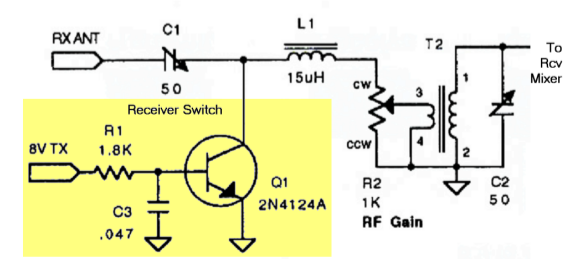
\includegraphics[scale=0.8]{./img/RxSwitch.png}
  \label{fig:RxSwitch}
  \caption{Receiver Switch}
\end{figure}

After the installation of the switching circuitry, the power amplifier was then
build according to the schematic shown in Figure~\ref{fig:powamp}.

\begin{figure}[h!]
  \centering
  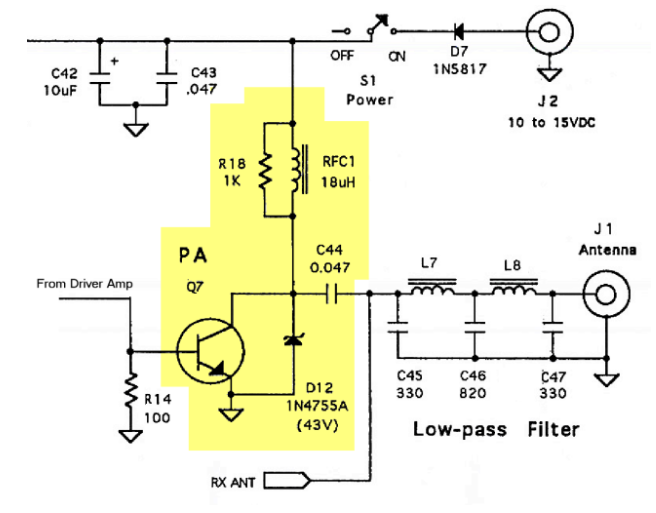
\includegraphics[scale=0.7]{./img/powamp.png}
  \label{fig:powamp}
  \caption{Power Amplifier}
\end{figure}

\subsection{Measurements}
In order to prevent cooking the oscilloscope, a 30dB attenuator was connected
between the antenna terminal and
%Ranging from 5V to 30V

\begin{tabular}{|c|c|c|c|c|}
  \hline
  Output Voltage $V_0$ & Output Power $P$  & Supply Power $P_0$  & Efficiency
  $\eta$\\
  \hline

\end{tabular}

\subsection{Plotting $\eta$ v.s. $P$}

In Figure~\ref{fig:efficiencyvpower}, the efficiency $\eta$ is plotted against the
output power $P$. In Figure~\ref{fig:gainvRFvolt}, the gain of the power
amplifier was plotted against the input RF Voltage.

\begin{figure}[h!]
  \centering
  %\includegraphics[scale=0.5]
    \label{fig:efficiencyvpower}
    \caption{Plot of Efficiency $\eta$ v.s. Output Power $P$}
\end{figure}

\begin{figure}[h!]
  \centering
  %\includegraphics[scale=0.5]
    \label{fig:gainvRFvolt}
    \caption{Plot of Gain v.s. input RF Voltage}
\end{figure}

\newpage
\section{Transmit Mixer}

Next, the Transmit Mixer was build and tested. Its schematic is shown in the
following Figure. 

\begin{figure}[h!]
  \centering
  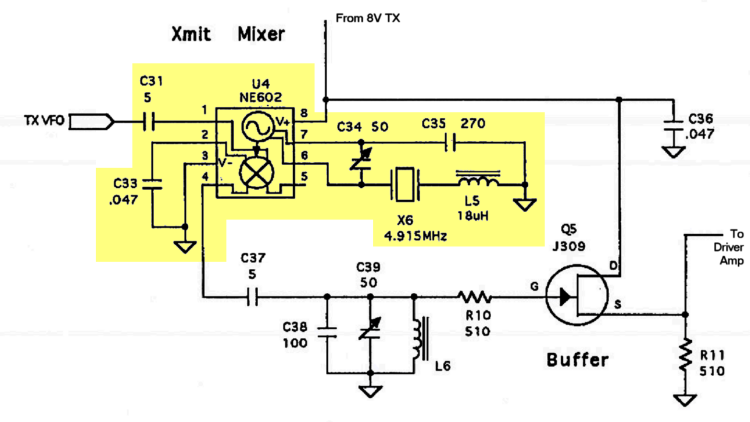
\includegraphics[scale=0.65]{./img/txmix.png}
\label{txmix}
\caption{Transmitter Mixer}
\end{figure}

\subsection{Initial Set of Measurements}

All components except $C_{31}$ were soldered. Next, $C_{34}$ was adjusted to get a
max voltage level at $\boxed{ V}$.
Next, the resonant frequency was measured across the crystal and inductor and
found to be $\boxed{ }$

%\begin{align*}
%  f_R&=\\
%  \therefore f_R&=\boxed{}
%\end{align*}

After these final measurements, $C_{31}$ was soldered in.

\end{document}

